% vim: set textwidth=78 autoindent:
% !TeX root = user_guide.tex

\chapter{Kern-Plugins verwenden}
\label{sec:core_plugins}
\index{Plugins!Kern-Plugins}

% when the revision of a chapter has been finalized, 
% comment out the following line:
%\updatedisclaimer

\begin{longtable}{|p{1.2cm}|p{3.8cm}|p{10.5cm}|}
\caption{23 QGIS Kern-Plugins}\label{tab:core_plugins} \\
\hline 
\textbf{Icon} & \textbf{Plugin} & \textbf{Beschreibung} \\
\endfirsthead
\hline
\textbf{Icon} & \textbf{Plugin} & \textbf{Beschreibung} \\
\endhead
\hline

\includegraphics[width=0.6cm]{delimited_text}
 & Layer aus Textdatei laden \index{Plugins!Layer aus Textdatei laden} & 
 CSV-Tabellen mit X- und Y-Koordinaten darstellen\\
\hline

\includegraphics[width=0.6cm]{coordinate_capture}
 & Koordinaten abgreifen \index{Plugins!Koordinaten abgreifen}& Koordinaten in
anderem KBS aus dem Kartenfenster abgreifen\\
\hline 
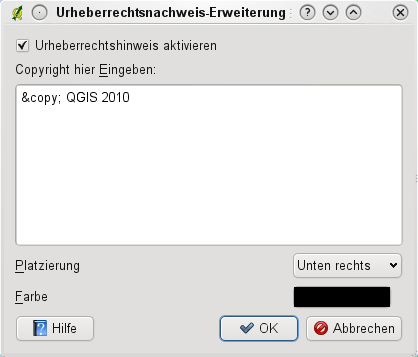
\includegraphics[width=0.6cm]{copyright_label}
 & Copyright Label \index{Plugins!Copyright}& Stellt
Urheberrechtsinformationen dar\\
\hline

\includegraphics[width=0.6cm]{diagram_overlay}
 & Diagram Overlay \index{Plugins!Diagram Overlay}& Diagramme oder Symbole
�ber Vektorlayern darstellen\\
\hline 

\includegraphics[width=0.6cm]{dxf2shp_converter}
 & DXF2Shape Konverter \index{Plugins!DXF2Shape Konverter}& Wandelt Daten vom DXF ins
Shapefile Format um\\
\hline
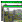
\includegraphics[width=0.6cm]{evis_icon}
 & eVis \index{Plugins!eVis}& Ereignisvisualisierungswerkzeug \\
\hline

\includegraphics[width=0.6cm]{ftoolslogo}
 & fTools \index{Plugins!fTools}& Analyse, Korrektur, Prozessierung und
Untersuchung von Shapes \\
\hline
% 
\includegraphics[width=0.6cm]{ftoolslogo}
 & GDAL Tools \index{Plugins!GDAL Tools} & GUI f�r GDAL Raster Tools \\
\hline

\includegraphics[width=0.6cm]{gps_importer}
 & GPS Werkzeuge \index{Plugins!GPS}& Werkzeuge zum Laden und Importieren von
GPS-Daten\\
\hline

\includegraphics[width=0.6cm]{grass}
 & GRASS \index{Plugins!GRASS Integration} & GRASS-Layer einer Location anzeigen
und bearbeiten\\
\hline
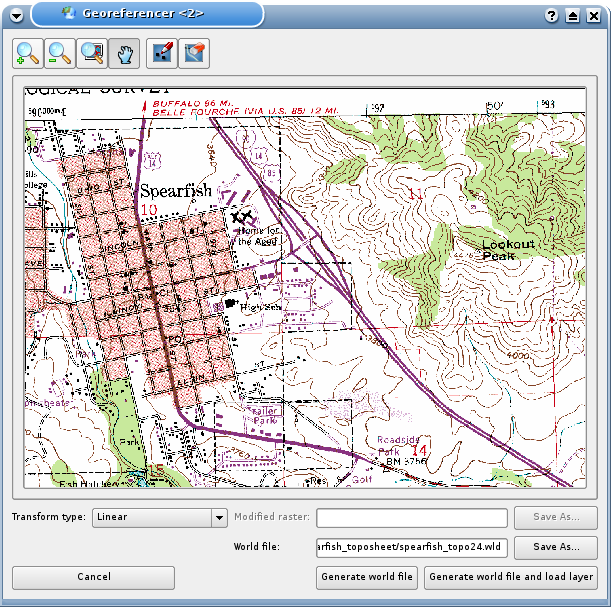
\includegraphics[width=0.6cm]{georeferencer}
 & GDAL-Georeferenzierer \index{Plugins!Georeferenzierer} & F�gt
Projektionsinformationen zu einer Rasterdatei hinzu\\
\hline

\includegraphics[width=0.6cm]{interpolation}
& Interpolationsplugin \index{Plugins!Interpolation}& Interpolation von
St�tzpunkten eines Vektorlayers in ein Raster\\
\hline

\includegraphics[width=0.6cm]{raster_terrain}
& Rastergel�ndeanalyse Plugin \index{Plugins!Rastergel�ndeanalyse} &
Rasterbasierte Gel�ndeanalysen\\
\hline

\includegraphics[width=0.6cm]{mapserver_export}
& MapServer Export \index{Plugins!MapServer Export}& Exportiert eine QGIS
Projektdatei in einen MapServer Mapfile \\
\hline
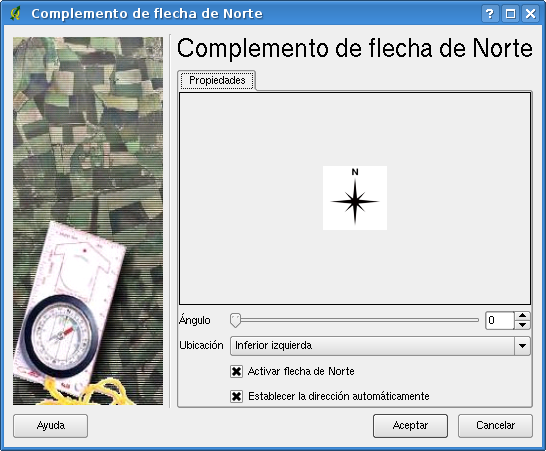
\includegraphics[width=0.6cm]{north_arrow}
& Nordpfeil \index{Plugins!Nordpfeil}& Stellt einen Nordpfeil im
Kartenfenster dar\\
\hline

\includegraphics[width=0.6cm]{ogr_converter}
 & OGR-Layer-Konverter \index{Plugins!OGR-Layer-Konverter} & OGR-unterst�tzte
Formate von einem in ein anderes umwandeln\\
\hline
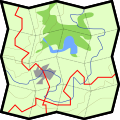
\includegraphics[width=0.6cm]{osm_icon}
 & OpenStreetMap \index{Plugins!OpenStreetMap} & Anzeigen und editieren von
OpenStreetMap Daten\\
\hline

\includegraphics[width=0.6cm]{oracle_raster}
 & Oracle Georaster \index{Plugins!Oracle Georaster} & Anbindung an Oracle
Georaster\\
\hline

\includegraphics[width=0.6cm]{plugin_installer}
 & Plugin Installer \index{Plugins!Plugin Installer} & Herunterladen und
installieren externer QGIS Python Plugins\\
\hline

\includegraphics[width=0.6cm]{spiticon}
 & SPIT \index{Plugins!SPIT}& Importieren von Shapefiles nach PostGIS \\
\hline

\includegraphics[width=0.6cm]{quick_print}
 & Schnelles Drucken \index{Plugins!Schnelles Drucken}& Ohne gro�en Aufwand eine
einfache Karte drucken \\
\hline
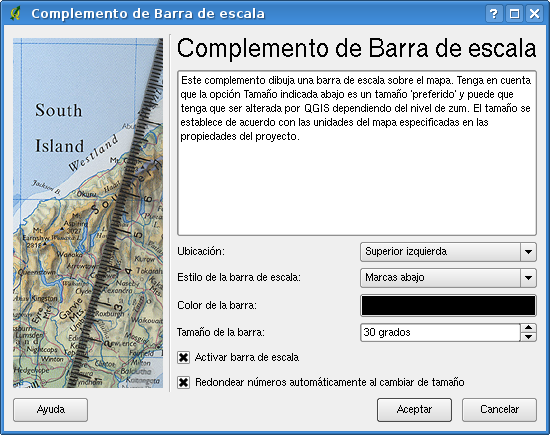
\includegraphics[width=0.6cm]{scale_bar}
 & Ma�stab \index{Plugins!Ma�stab}& Zeichnet einen Ma�stab ins Kartenfenster\\
\hline

\includegraphics[width=0.6cm]{mIconAddWfsLayer}
 & WFS-Plugin \index{Plugins!WFS} & L�dt und stellt WFS-Layer dar \\
\hline
\end{longtable}


